%MIT OpenCourseWare: https://ocw.mit.edu
%RES.18-011 Algebra I Student Notes, Fall 2021
%License: Creative Commons BY-NC-SA 
%For information about citing these materials or our Terms of Use, visit: https://ocw.mit.edu/terms.

\section{Symmetry Groups}

So far, in this class, we've covered \emph{groups} and \emph{linear algebra}. Now, we are looking at groups of symmetries that preserve extra forms of structure. 

\subsection{Review}
Last week, we looked at the \emph{orthogonal matrices}. 
 
\begin{definition}
The \textbf{orthogonal matrices} $O_n$ are matrices that preserve \emph{distance}. It is the set 
\[
T: \RR^n \rto \RR^n : |Tv| = |v| \text{ for all } v \in \RR^n.
\]
\end{definition}

\begin{definition}
The set $M_n$ of \textbf{isometries} from $\RR^n$ to itself is 
\[
\{f: \RR^n \rto \RR^n : |f(u)-f(v)| = |u-v|\}.
\]
\end{definition}

The orthogonal matrices are the subset of isometries that are \emph{linear transformations.} In class, we showed that every isometry $f$ is of the form $f(x) = Ax + b$ where $A \in O_n$ and $b \in \RR^n.$

Then, we looked at $O_2,$ the orthogonal matrices in two dimensions. There are two possibilities for a transformation in $O_2.$
\begin{itemize}
    \item Rotations around $0$: these have determinant 1 and are called $SO_2$. \footnote{The special orthogonal group}
    \item Reflections across a line through $\vv{0}$: these have determinant -1
\end{itemize}

Then the \emph{isometries} of two-dimensional space, $M_2,$ also fit into several categories.\footnote{This is quite surprising, since a priori, an isometry could take many different forms.}
\begin{itemize}
    \item Translations
    \item Rotations around $p$ 
    \item Reflections across a line
    \item A glide reflection\footnote{A reflection in addition to a parallel translation}
\end{itemize}

\subsection{Examples of Symmetry Groups}
Now, we want to add some additional structure to preserve.

\begin{qq}
What isometries of $\RR^2$ fix some shape inside $\RR^2$?
\end{qq}

We call the group of such isometries \emph{symmetry groups} for that shape. Let's start with a couple examples of shapes and their symmetry groups. 
\begin{example}
For a regular pentagon, the group of symmetries are rotations by multiples of $\frac{2\pi}{5}$, and reflections across lines. This group of symmetries is what we would call \emph{discrete}.\footnote{This will be formalized later on.}
\begin{center}
    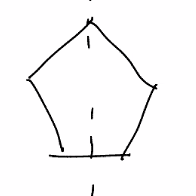
\includegraphics[width=3cm]{Lecture Files and Images/lec14-pentagon.png}
\end{center}
\end{example}
Next, we look at a group that is not discrete.
\begin{example}
For a circle centered at the origin, every rotation or reflection will fix it, and so its symmetry group is all of $O_2.$ This group of symmetries is \emph{not discrete}.
% \begin{center}
%     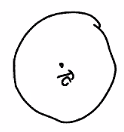
\includegraphics[width=3cm]{images/lec14-circle.png}
% \end{center}  %\todo put the graphics back in
\end{example}
We can also look at infinitely large shapes. 
\begin{example}
For a triangular lattice, certain translations, reflections over lines, rotations, and glide reflections all preserve it. It is a \emph{discrete} symmetry group.
\begin{center}
    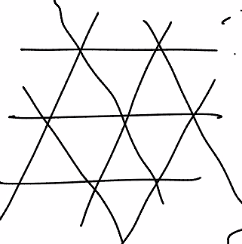
\includegraphics[width=3cm]{Lecture Files and Images/lec14-trianglelattice.png}%\todo add in picture of glide reflection from lecture notes
\end{center}
\end{example}

\subsection{Discrete Subgroups of \texorpdfstring{$\RR$}{R}}
From our examples, we see that some symmetry groups are ``discrete" and some are not.
\begin{qq}
How can the notion of a \emph{discrete group} be formalized?
\end{qq}
We can start with an easier notion, which is a discrete group inside $(\RR, +).$
\begin{definition}
A group $G \leq (\RR, +)$ is discrete if there exists $\varepsilon > 0$ such that any $g \in G$ such that $g \neq 0$ satisfies $|g| > \varepsilon.$ Equivalently, for $a, b \in G$ and $a \neq b,$ then it must be true that $|a-b| > \varepsilon$ for a discrete group. 
% \begin{center}
%     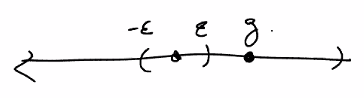
\includegraphics[width=3cm]{images/lec14-discrete.png}
% \end{center} %\todo{put the graphics back in}
\end{definition}

The discreteness tells us some important information about $G.$
\begin{theorem}\label{discrete subgroups of r}
If $G \leq (\RR, +)$ is discrete, then $G = \{0\}$ or $G = \ZZ \alpha$ for some real number $\alpha > 0.$ 
\begin{center}
    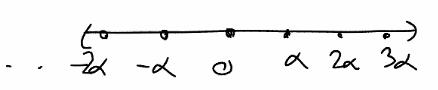
\includegraphics[width=5cm]{Lecture Files and Images/lec14-disc.png}
\end{center} %\todo put the graphics back in
\end{theorem}
This theorem is very similar to the theorem we had about subgroups of $\ZZ,$ where we showed they were either trivial or of the form $k\ZZ$.
\begin{proof}
Assume that $G \neq \{0\}.$ Then there is some smallest positive element $\alpha \in G.$ 
To see why it is possible to find a smallest element, we start by taking any $g > 0$ in $G$. 
By discreteness, in the interval from $[0, g]$, we have at most $g/\varepsilon$ elements of $G$ inside of the interval. 
We can then pick the smallest one because the set is finite.

We now claim that $G = \ZZ \alpha.$ Why is this true? If $2\alpha < x < 3\alpha$ for some $x \in G,$ then $0 < x-2\alpha < \alpha,$ where $x-2\alpha \in G,$ which is a contradiction.
\footnote{The discreteness guarantees that we can find a smallest positive element! This is definitely \emph{not} the case for $\RR$ in general (it is a fundamental property of $\RR$ that there is \emph{no} smallest positive element.)}
\end{proof}

\subsection{Finite subgroups of \texorpdfstring{$O_2$}{O2}}
So what are all the finite subgroups of $O_2?$ 
Let's first try to create some examples to get some intuition about them.
\begin{example}
Let $x$ be a rotation by $\frac{2\pi}{n}.$ Then $C_n = \langle x \rangle$\footnote{$\{1, x, \cdots, x^{n-1}\}$}, the cyclic group of order $n,$ is generated by $x$, and is a finite subgroup of $O_2.$ 
\end{example}

Another possible finite subgroup can be created by expanding $C_n$ a little bit. 
\begin{example}
Let $y$ be a reflection across a line $\ell$ through $\vv{0}.$ Notice that the relations $yx = x^{-1}y, y^2 = e,$ and $x^n = e$ hold, and so any product  $y^{a_1}x^{a_2}y^{a_3}\cdots$ can be written as $x^{i}y^{j},$ where $0 \leq i < n$ and $0 \leq j < 2.$ Then the group generated by $x$ and $y$ is 
\[
D_n \coloneqq \langle x, y \rangle = \{e, x, x^2, \cdots, x^{n-1}, y, xy, x^2y, \cdots, x^{n-1}y\},
\]
which is called the dihedral group. It has order $2n.$
\end{example}

For $n \geq 3,$ $D_n$ is the group of symmetries of a regular $n-$gon.\footnote{In general, if $x$ is a rotation by an angle that is not a rational multiple of $2\pi,$ then we do not get a rational group. We would get a non-discrete subgroup of $SO_2.$} The dihedral group for $n= 1$ is $D_1 \cong C_2$ and for $n = 2$, $D_2 \cong C_2 \by C_2.$ For $n=3,$ $D_3 \cong S_3,$ and larger dihedral groups can also be studied. 

Now, we have two families of finite subgroups of $O_n$, the cyclic groups of rotations, and the dihedral groups. It turns out that these are actually all the finite subgroups of $O_2$. This provides yet another classification theorem.

Let's start with a simpler version. 
\begin{theorem}
If a subgroup $H \leq SO_2$ is finite, then $H$ is isomorphic to $C_n$ for some $n.$
\end{theorem}
\begin{proof}
Let $\rho_{\theta}$ be $\begin{pmatrix}
\cos\theta & -\sin\theta \\
\sin\theta & \cos\theta
\end{pmatrix}$. Then let
\[
S = \{\theta \in \RR \text{ such that } \rho_{\theta} \in H\}.
\]

Under the homomorphism $\pi: \theta \mapsto \rho_{\theta}$, $S = \pi^{-1}(H).$ Since $S$ is a preimage, we know that $S$ is a subgroup of $(\RR, +)$.

If $H$ is finite, then $S$ must be discrete, and so by Theorem \ref{discrete subgroups of r}, $S$ is $\ZZ \alpha$ for some $\alpha.$ Also, $2\pi \in S$ because a rotation by $2\pi$ is the identity in $H$, and so $\alpha = \frac{2\pi}{n}$. So $\boxed{H= C_n.}$ 
\end{proof}

\begin{theorem}\label{everything is cn or dn}
Any finite subgroup of $O_2$ is isomorphic to $C_n$ or $D_n.$ 
\end{theorem}
Now, we can prove Theorem \ref{everything is cn or dn}. 
\begin{proof}
There are two cases:
\begin{itemize}
    \item \textbf{Case I.} If $G \subseteq SO_2,$ by the above theorem, $G \cong C_n$ for some $n.$
    \item \textbf{Case II.} If $G$ is not a subset of $SO_2,$, then take the restriction of the determinant function on $O_2$ to $G.$ It takes \[G \xrightarrow[]{\det}\{\pm 1\}.\] By the assumption that $G$ isn't a subset of $SO_2,$ this is surjective. Let 
    \[
    H = \ker(G \xrightarrow[]{\det}\{\pm 1\}).
    \]
    Then, $H \nsub G$ is a normal subgroup of index 2. So $\det^{-1}(\{-1\})$ is a nontrivial coset of $H,$ and so it is $Hr$ for some $r \in G$ such that $\det(r) = -1.$ Then $r$ must be a reflection across some line $\ell.$\footnote{Note that we have many options for $\ell$ because any $r\in Hr$ generates $Hr$. In particular, these are all the rotations of $\ell$.} Then, it is clear by definition that $H \leq SO_2,$ and so $H = C_n$ for some $n,$ and it is generated by some $x = \frac{2\pi \rho}{n}$, and then we have 
    \[
    G = \left \langle \frac{2\pi\rho}{n}, r\right \rangle \cong D_n.
    \]
\end{itemize}
\end{proof}

\subsection{More Discrete Subgroups}
Next, what are the finite or discrete subgroups of $M_2$? Let's start with a couple of definitions. 

\begin{definition}
A subgroup $G \leq O_2$ is \textbf{discrete} if there exists some $\varepsilon > 0$ such that all nontrivial rotations in $G$ have angle $\theta$ such that $|\theta| > \varepsilon.$\footnote{Here, discrete implies finite, which implies that it is $C_n$ or $D_n.$}
\end{definition}

\begin{definition}
A subgroup $G \leq M_2$ is \textbf{discrete} if there exists some $\varepsilon > 0$ such that all translations in $G$ are by vectors $b$ with $|b| > \varepsilon,$ and all rotations in $G$ have angle $\theta$ such that $|\theta| > \varepsilon.$
\end{definition}

This ends up being quite a strong constraint on what the discrete subgroups look like, even though there could be lots of different possibilities. We'll talk about this more next time.

\newpage